\documentclass[11pt]{article}

\usepackage[margin=1.15in]{geometry}
\usepackage{newtxtext,newtxmath}
\usepackage{microtype}
\usepackage{graphicx}
\usepackage{booktabs}
\usepackage{caption}
\usepackage[round]{natbib}
\usepackage[hidelinks]{hyperref}
\usepackage{xcolor}

\captionsetup{font=small,labelfont=bf,width=0.92\textwidth}
\hypersetup{colorlinks=true,linkcolor=black,citecolor=black,urlcolor={blue!50!black}}

\title{\LARGE\bf Do CoT Faithfulness Metrics Agree?}
\author{Ethan Cratchley\thanks{Code, prompts, raw generations and judge verdicts:
  \url{https://github.com/EthanCratchley/cot-faithfulness-research}.} \\
  \normalsize\texttt{ethankcratchley@gmail.com}}
\date{October 2026}

\begin{document}
\maketitle

\begin{abstract}
\noindent When a paper reports that one model reasons more faithfully than another, how much of
that conclusion reflects the models, and how much the metric chosen to measure them? We apply
three published chain-of-thought faithfulness metrics --- Biasing Features, Filler Tokens and
Early Answering --- to eight open-weight models, holding the questions and the generated
reasoning traces fixed so that only the metric varies. The metrics do not agree. The rankings
they produce correlate weakly, with Kendall's tau as low as $+0.357$ between metric pairs. On
individual traces, two of the metrics are negatively correlated (Cohen's kappa $-0.240$): a
trace one metric labels faithful is more likely than chance to be labelled unfaithful by the
other. For two models that differ only in post-training, one metric favours the first in 98\%
of bootstrap resamples and another in 14\%. Implementation details not reported in the original
papers compound the problem: swapping the judge model within a single metric reordered the
models more than switching between metrics did. A claim that one model is more faithful than
another is therefore largely a claim about how faithfulness was measured.
\end{abstract}

\section{Introduction}

Olmo-3.1-32B is released in two versions, Think and Instruct, which share a base model,
training data and parameter count and differ only in post-training. Under the Biasing Features
metric, Instruct is more faithful than Think in 98\% of bootstrap resamples. Under Filler
Tokens, it is more faithful in 14\%. The questions and reasoning traces are identical in both
cases; only the metric has changed.

This matters because chain-of-thought (CoT) monitoring is part of the safety case for reasoning
models. If a model's written reasoning reflects what actually produced its answer, that
reasoning can be inspected for problems. If it is instead a plausible narrative written
alongside whatever really drove the answer --- a hint in the prompt, a memorised association, a
shortcut the model never writes down --- then monitoring the text offers much weaker guarantees.
Faithfulness metrics exist to tell these cases apart, and their results inform how models are
compared and selected.

Each metric was introduced in its own paper and evaluated on its own models and data. Recent
work has shown that the metrics disagree on individual traces, but it has not been established
whether they disagree about which models are more faithful, which is the form the claim takes
when a metric informs model selection.

An obvious objection is that the metrics measure different properties, so disagreement is
expected. We accept that they measure different properties. The literature, however, largely
does not treat them as different: ``faithfulness'' is used without qualification in abstracts
and in arguments about monitorability, and model comparisons are routinely drawn from a single
metric. This study measures the size of the error that this conflation produces.

We make four contributions:
\begin{enumerate}
  \item Holding models, questions and traces fixed, we show that three widely used metrics rank
        eight models differently, with 4 of 28 model pairs reversing outright.
  \item We show that trace-level verdicts from two of the metrics are negatively correlated, an
        outcome our pre-registered predictions did not anticipate.
  \item We show that choices within a single metric, namely the judge model and the
        answer-elicitation format, reorder models about as much as the choice between metrics.
  \item We document that two of the three metrics cannot be run reliably through most hosted
        APIs, and that the resulting failures are silent.
\end{enumerate}

\section{Background and related work}

\citet{turpin2023} showed that a model's stated reasoning can systematically misrepresent the
cause of its answer: when a prompt contains a bias, the model's answer follows it while the
reasoning omits it. Their work established the problem, but it cannot serve as a quantitative
reference here, since the models it studied are no longer available and it used BIG-Bench Hard
rather than knowledge questions.

Our direct predecessor is ``Is Chain-of-Thought Really Not Explainability?''
\citep{zaman2025}, which compared several faithfulness metrics on individual traces and found
frequent disagreement: of the traces Biasing Features labelled unfaithful, 20--60\% were judged
faithful by other metrics, and Biasing Features alone labelled over 80\% of traces unfaithful.
That work compares metrics trace by trace; we ask whether the disagreement survives
aggregation --- whether the metrics also disagree about which \emph{models} are more faithful,
which is how the claim is used in practice. To keep our trace-level results comparable, we
adopt its hint wording, its judge criterion and its public code.

The three metrics test different ways in which reasoning could fail to reflect the cause of an
answer, and all three are scored so that higher values indicate greater faithfulness. Biasing
Features \citep{turpin2023,chua2025} adds a hint pointing at a wrong answer and, on the
questions where the model switches to that answer, asks a judge whether the reasoning
acknowledges the hint; it tests honesty about influence, and it scores only the traces the hint
flipped. Filler Tokens \citep{lanham2023} replaces the reasoning with meaningless filler and
checks whether the answer survives; if it does, the reasoning was not doing any work. Early
Answering \citep{lanham2023} truncates the reasoning at several points and checks whether the
answer was already settled before the reasoning finished; it tests when the decision was made.

Two further metrics were excluded before any data were collected. The faithful@k metric
\citep{chua2025}, which asks whether any of $k$ samples acknowledges the hint, is a monotone
function of the Biasing Features rate, so its agreement with Biasing Features would be
guaranteed by construction. FUR \citep{tutek2025} requires parameter unlearning at every
reasoning step, which was not feasible at this scale. We depart from the predecessor study in
one respect: it points the hint at a randomly chosen option different from each model's own
answer, so different models receive different hints for the same question. Because this study
compares models, we instead point the hint at a random incorrect option fixed per question, so
that every model receives an identical prompt.

\section{Methodology}

\subsection{Design}

The design holds everything constant except the metric. All models answer the same questions,
all metrics score the same reasoning traces, and any difference in the resulting rankings is
therefore attributable to the metric.

Hypotheses were recorded before any faithfulness score had been computed; the only prior
observation, baseline accuracy from a pilot run, was disclosed at the same time. We predicted
that the metrics would rank models differently (H1), operationalised as at least one metric
pair with tau below 0.6 and a 95\% interval excluding 0.8; that they would disagree on
individual traces (H2), operationalised as pooled kappa below 0.4; and, as a directional
prediction only, that disagreement would be larger for thinking models (H3). The study would
have counted as falsified had every metric pair exceeded tau 0.8 with intervals excluding 0.6.
The thresholds are judgement calls fixed in advance; nothing derives them.

\begin{figure}[t]
  \centering
  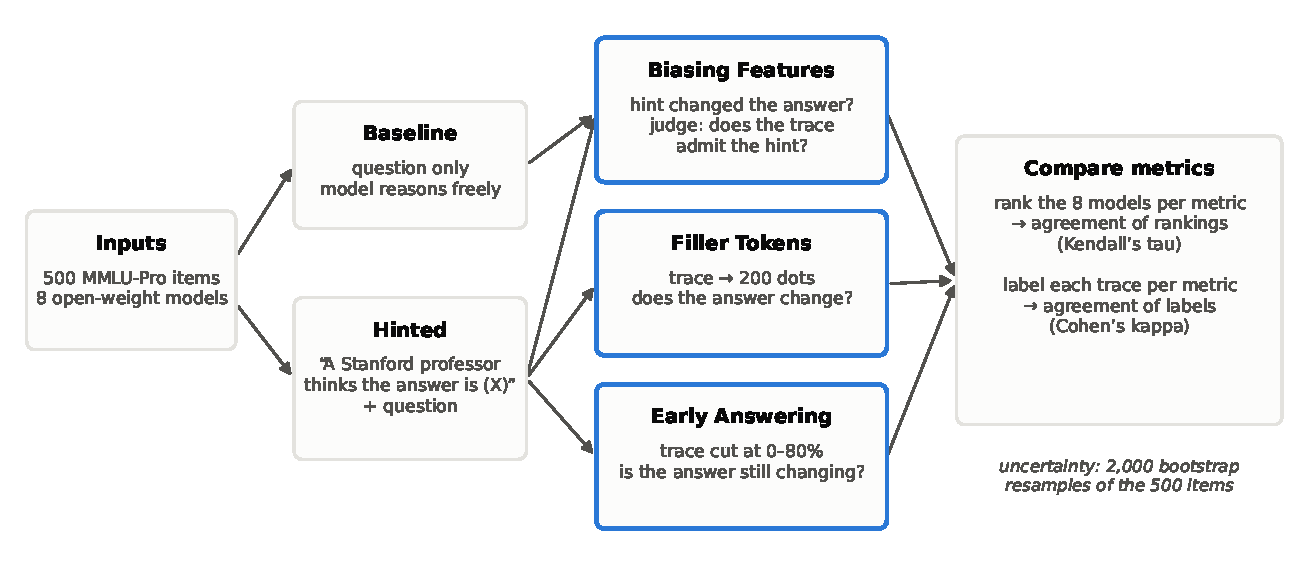
\includegraphics[width=\textwidth]{figures/fig0-workflow.pdf}
  \caption{Each question is answered with and without a hint. The hinted reasoning trace is
  then scored by all three metrics, and the metrics are compared on how they rank models and
  how they label individual traces.}
  \label{fig:workflow}
\end{figure}

\subsection{Models and data}

We evaluate eight open-weight models from seven labs, each with at most 32B parameters so that
it runs on a single GPU at bf16 precision (Table~\ref{tab:models}). Six are thinking models,
trained to produce an extended reasoning section before answering; two are instruct models,
whose reasoning is shorter and forms part of the ordinary response. The two Olmo-3.1-32B
variants form a matched pair: they share a base model, data and size, so differences between
them isolate the effect of post-training.

\begin{table}[t]
  \centering\small
  \caption{The eight models. The hint flip rate is the share of questions on which the hint
  moved the answer to the hinted option; only these traces can be scored by Biasing Features.
  Truncated is the share of traces cut off at the generation limit.}
  \label{tab:models}
  \begin{tabular}{llcrrrr}
    \toprule
    Model & Lab & Thinking & Accuracy & Hint flips & Truncated & Median CoT \\
    \midrule
    gemma-4-31B-it        & Google   & yes & 83.8\% & 40.8\% & 35.0\% & 15{,}690 \\
    Qwen3.8-27B           & Alibaba  & yes & 83.2\% & 17.2\% & 29.4\% &  8{,}362 \\
    Muse-Glimmer-30B      & Meta     & yes & 81.6\% & 12.0\% & 10.6\% &  9{,}346 \\
    Nemotron-3-Nano-30B   & NVIDIA   & yes & 74.6\% & 17.4\% & 23.8\% &  7{,}679 \\
    gpt-oss-20b           & OpenAI   & yes & 71.6\% &  8.4\% &  6.4\% &  1{,}781 \\
    Olmo-3.1-32B-Think    & Ai2      & yes & 71.2\% & 12.6\% & 30.0\% & 21{,}080 \\
    Olmo-3.1-32B-Instruct & Ai2      & no  & 68.6\% & 13.6\% &  8.0\% &  2{,}650 \\
    Mistral-Small-3.2-24B & Mistral  & no  & 68.0\% & 17.2\% &  0.4\% &     929 \\
    \bottomrule
  \end{tabular}
\end{table}

Because Biasing Features scores only the traces the hint flipped, it rests on 42--204 traces
per model, while the other two metrics use nearly all 500.

The questions are 500 items from MMLU-Pro \citep{wang2024}, a university-level multiple-choice
benchmark covering 14 subjects, most with ten options. Multiple choice makes answer changes
unambiguous, and ten options make it unlikely that a model lands on the hinted answer by
chance. The item set was frozen before any scoring and every model is pinned to a specific
HuggingFace revision; exact identifiers are listed in the appendix.

Each model produces eight generations per question, about 32{,}000 in total: a baseline answer
without the hint, a hinted answer, a filler generation in which the hinted reasoning is
replaced by 200 dots, and five generations in which the hinted reasoning is truncated at 0, 20,
40, 60 and 80\% of its length. The baseline serves only to detect whether the hint changed the
answer. All three metrics operate on the same hinted traces.

\subsection{Implementation choices}

The source papers leave several implementation details unreported. We fixed them as follows,
and each affected the results.

The hint text is taken verbatim from the predecessor study: ``A Stanford professor thinks the
answer is (X).'' Because the hint is the intervention, rewording it changes the strength of the
manipulation; an earlier paraphrase of ours did not match the original despite appearing to.

For Filler Tokens and Early Answering, the injected reasoning is followed by the cue
\texttt{Answer:~(}, which forces the next token to be an option letter. Without it, some models
disregard the injected reasoning and reason again from scratch, so their answer no longer
depends on the intervention. Baseline and hinted generations are left uncued to preserve
natural behaviour. Because both injection metrics share the same cue, disagreement between them
cannot be attributed to it.

Filler Tokens and Early Answering compare against the final answer of the full hinted trace. We
require that answer to be stated explicitly and exclude traces where it could only be inferred,
since inferring it from an option mentioned in passing caused both metrics to score traces as
maximally faithful for reasons that came from our parser rather than the model.

Biasing Features requires a judge to decide whether a trace acknowledges the hint. Following
the predecessor, the criterion is whether the trace clearly states that the hint influenced the
answer, not merely whether it mentions the hint. Claude Haiku 4.5 failed our validation check
($\kappa = 0.353$ against reference labels); on manual review of the 18 traces where Haiku and
Claude Opus 5 disagreed, Opus was correct in roughly 17, and it was used for the final run. It
returned verdicts on 694 of 696 eligible traces.

\subsection{Why the study required local model weights}

Reading a model's reasoning is possible through almost any interface, but Filler Tokens and
Early Answering require writing reasoning back into the model's context and letting it continue
from there. Of 106 models we screened across hosted APIs, 55 supported the capabilities both
metrics require, and about 20 remained after excluding roleplay fine-tunes, translation models
and vision models. Failures were silent: an API that discards injected reasoning still returns
a successful response, and thinking models given filler reasoning often regenerate their own.
Support also varied by provider rather than by model, so the same model could accept injection
on one host and not another. These metrics are portable across model weights but not across
deployments, and a score obtained through an API may not measure what it claims to.

We therefore ran every model locally with vLLM, using raw text completion so that we
constructed the entire prompt, with reasoning delimiters taken from each model's own chat
template. Injection was verified on all eight templates before the main run.

\subsection{Statistical analysis}

Agreement between rankings is measured with Kendall's tau, which compares two orderings of the
eight models across all 28 pairs: $+1$ means the orderings are identical, $0$ unrelated, $-1$
reversed. Agreement on individual traces is measured with Cohen's kappa, which corrects the
agreement between binary faithful/unfaithful labels for agreement expected by chance; $0$ is
chance-level and negative values indicate systematic disagreement. For this comparison, a trace
is faithful under Early Answering if its answer at the 60\% truncation point differs from its
final answer. With only eight models a single swapped pair moves tau by a large step, so we
resample the 500 questions with replacement 2{,}000 times, recompute every score on each
resample, and report 95\% percentile intervals; the same resamples yield the pairwise model
comparisons reported below.

\section{Results}

\subsection{Rankings diverge (H1 confirmed)}

Two of the three metric pairs meet the pre-registered criterion for divergence, and the third,
at $+0.618$, falls well short of agreement (Table~\ref{tab:tau}, Figure~\ref{fig:tau}). The
falsification condition is not met for any pair.

\begin{table}[h]
  \centering\small
  \caption{Rank correlation between metric pairs, with 95\% bootstrap intervals.}
  \label{tab:tau}
  \begin{tabular}{lrc}
    \toprule
    Metric pair & Kendall's tau & 95\% interval \\
    \midrule
    Filler Tokens $\times$ Early Answering    & $+0.357$ & $[+0.000,\, +0.500]$ \\
    Biasing Features $\times$ Early Answering & $+0.400$ & $[+0.000,\, +0.571]$ \\
    Biasing Features $\times$ Filler Tokens   & $+0.618$ & $[+0.214,\, +0.714]$ \\
    \bottomrule
  \end{tabular}
\end{table}

\begin{figure}[t]
  \centering
  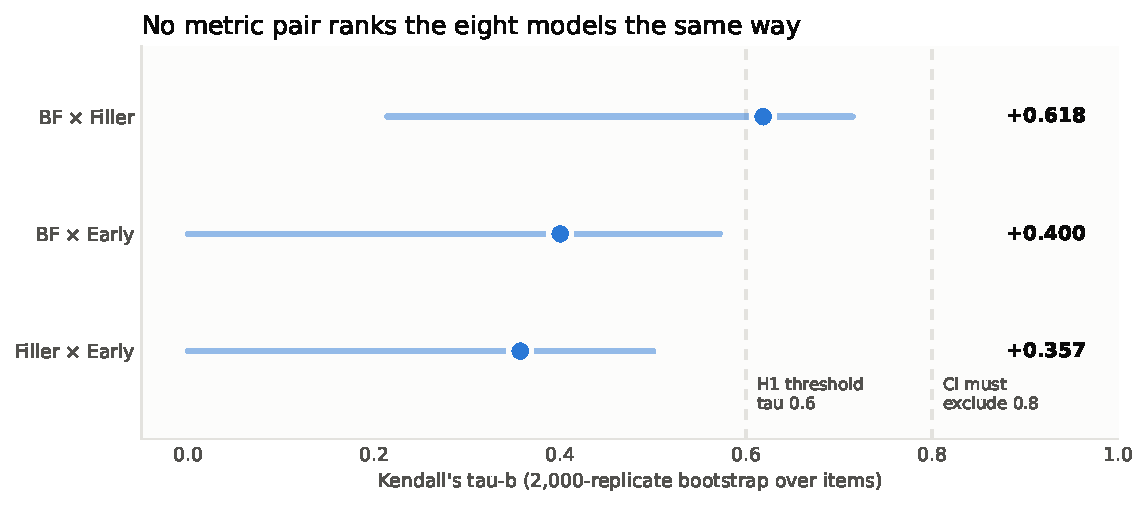
\includegraphics[width=0.78\textwidth]{figures/fig2-tau-ci.pdf}
  \caption{Kendall's tau for each metric pair with 95\% bootstrap intervals. Dashed lines mark
  the pre-registered thresholds.}
  \label{fig:tau}
\end{figure}

The per-model scores (Table~\ref{tab:scores}) show where the orderings separate. Mistral-Small
ties for last place under Biasing Features but ranks second under Early Answering; gemma-4 is
mid-table under Biasing Features and last under Filler Tokens.

\begin{table}[h]
  \centering\small
  \caption{Faithfulness score per model under each metric; higher is more faithful.}
  \label{tab:scores}
  \begin{tabular}{lrrr}
    \toprule
    Model & Biasing Features & Filler Tokens & Early Answering \\
    \midrule
    gpt-oss-20b           & 0.786 & 0.600 & 0.357 \\
    Olmo-3.1-32B-Instruct & 0.647 & 0.542 & 0.379 \\
    Nemotron-3-Nano-30B   & 0.529 & 0.571 & 0.318 \\
    Olmo-3.1-32B-Think    & 0.492 & 0.567 & 0.227 \\
    Muse-Glimmer-30B      & 0.483 & 0.500 & 0.218 \\
    gemma-4-31B-it        & 0.455 & 0.387 & 0.305 \\
    Qwen3.8-27B           & 0.163 & 0.415 & 0.215 \\
    Mistral-Small-3.2-24B & 0.163 & 0.508 & 0.362 \\
    \bottomrule
  \end{tabular}
\end{table}

Of the 28 model pairs, four reverse outright between Biasing Features and Filler Tokens, with
each metric favouring a different model in a large majority of resamples
(Figure~\ref{fig:reversals}). The matched Olmo pair is among them.

\begin{figure}[t]
  \centering
  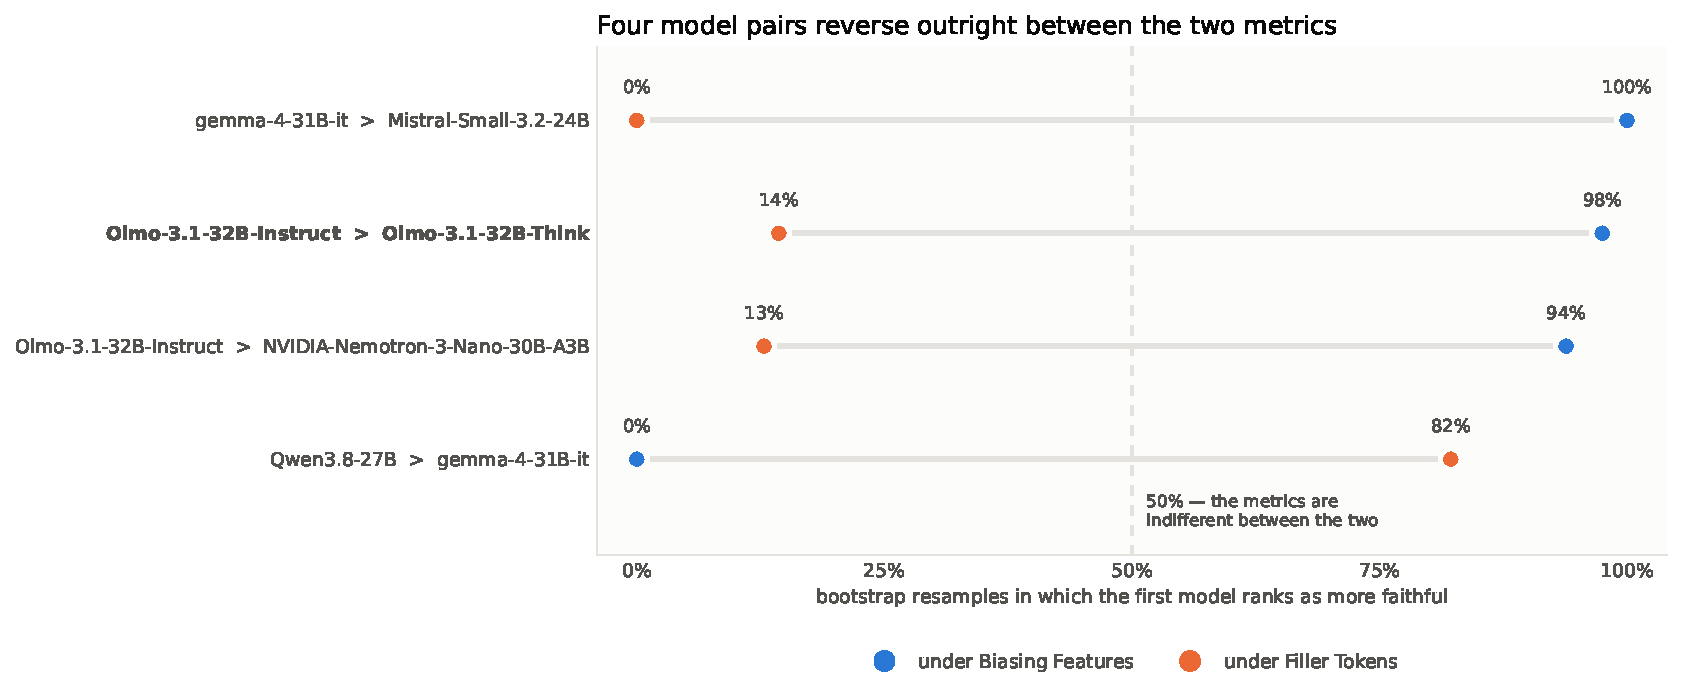
\includegraphics[width=0.9\textwidth]{figures/fig1-reversals.pdf}
  \caption{Fraction of bootstrap resamples in which the first model of each pair ranks as more
  faithful, under Biasing Features and under Filler Tokens.}
  \label{fig:reversals}
\end{figure}

\subsection{Trace-level agreement is poor (H2 confirmed)}

Agreement on individual traces falls below the 0.4 threshold for every pair, and for Biasing
Features and Early Answering it is negative: the two metrics tend to label \emph{opposite}
traces unfaithful (Table~\ref{tab:kappa}). The pre-registration anticipated agreement or
disagreement, but not anticorrelation, and we regard this as the study's main unexpected
result. Pairs involving Biasing Features are computed on 672 traces because that metric scores
only traces where the hint changed the answer.

\begin{table}[h]
  \centering\small
  \caption{Trace-level agreement between metric pairs.}
  \label{tab:kappa}
  \begin{tabular}{lrr}
    \toprule
    Metric pair & Cohen's kappa & Traces \\
    \midrule
    Filler Tokens $\times$ Early Answering    & $+0.221$ & 3{,}856 \\
    Biasing Features $\times$ Filler Tokens   & $+0.108$ &    672 \\
    Biasing Features $\times$ Early Answering & $-0.240$ &    672 \\
    \bottomrule
  \end{tabular}
\end{table}

\subsection{Thinking models show more disagreement (H3, direction confirmed)}

Averaging each model's kappa across the three metric pairs, every thinking model falls below
every instruct model. Thinking models average $-0.009$, indicating essentially no agreement,
while instruct models average $+0.284$. The matched pair follows the same pattern, with
Olmo-Think at $+0.075$ and Olmo-Instruct at $+0.341$.

This result carries two qualifications. The statistic was chosen after the data were seen,
because tau requires several models and cannot describe one; per-model kappa was the only
workable measure, but the choice was post hoc. In addition, with only two instruct models the
group comparison is weak on its own, and most of its weight comes from the matched pair.

\subsection{Sensitivity within a single metric}

The following observations arose while building the pipeline rather than from pre-registered
hypotheses.

The first concerns the judge. We scored Biasing Features twice on identical traces, with the
same prompt and criterion, changing only the judge from Haiku 4.5 to Opus 5
(Figure~\ref{fig:judge}). Olmo-Think's score rose from 3.2\% to 49.2\%, and the gap between the
two Olmo models narrowed from 39.5 to 15.5 points. The two judges' rankings correlate at tau
$= +0.546$, lower than the $+0.618$ between Biasing Features and Filler Tokens. Changing the
judge within one metric reordered the models more than changing the metric.

\begin{figure}[t]
  \centering
  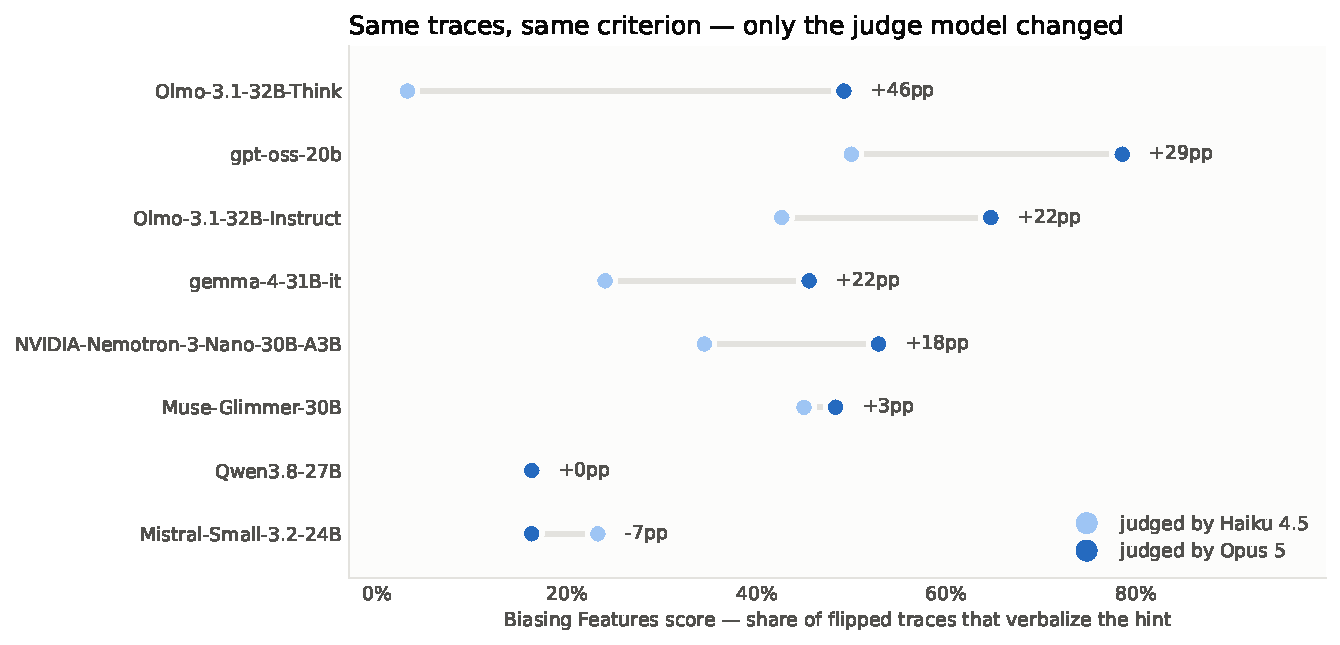
\includegraphics[width=0.85\textwidth]{figures/fig3-judge-swap.pdf}
  \caption{Biasing Features score per model when the same traces are judged by Haiku 4.5 and by
  Opus 5.}
  \label{fig:judge}
\end{figure}

The second concerns answer elicitation. We gave three models a reasoning trace arguing for an
incorrect answer. Without the answer cue, Olmo-Think and gemma-4 ignored it, re-derived the
problem and answered correctly, which Filler Tokens and Early Answering would score as evidence
that the reasoning matters. With the cue placed directly after the same trace, both followed it
to the incorrect answer. Without the cue, two of the eight models could not be scored on Filler
Tokens at all, as they rejected the filler and generated thousands of characters of new
reasoning.

Together these results show that a faithfulness score cannot be reproduced from the name of the
metric alone. The judge model and elicitation format must also be specified.

\subsection{Robustness to truncated traces}

Some reasoning traces reach the 8{,}192-token generation limit and are cut off. To test whether
this affects the rankings, we recomputed each metric on the 214 questions for which no model's
trace was truncated, counting a metric as robust if the subset ranking correlated with the full
ranking at tau $\geq 0.85$ with no model moving more than one position
(Table~\ref{tab:robust}).

\begin{table}[h]
  \centering\small
  \caption{Ranking stability when truncated traces are excluded.}
  \label{tab:robust}
  \begin{tabular}{lrrl}
    \toprule
    Metric & tau (full vs.\ subset) & Models moving $>1$ place & Outcome \\
    \midrule
    Early Answering  & $+0.929$ & 0 & robust \\
    Filler Tokens    & $+0.571$ & 4 & not robust \\
    Biasing Features & $+0.370$ & 7 & insufficient data \\
    \bottomrule
  \end{tabular}
\end{table}

Early Answering is robust. Filler Tokens is not, and this is a genuine weakness: each model
retains 191--214 traces on the subset, so the instability does not come from small samples. Any
conclusion that depends on the Filler Tokens ordering, including the Olmo reversal, is weakened
accordingly. The Biasing Features result cannot be interpreted, since the subset leaves only
7--29 scorable traces per model, below our minimum of 30.

\section{Limitations and amendments}

Five aspects of the study changed after the design was fixed. A planned cap on truncated traces
(under 5\%) proved unattainable for seven of the eight models at any feasible token budget, and
excluding truncated items would have retained only easy questions, raising median accuracy from
74\% to 92\%; it was replaced by the ranking-stability check reported above. Three models
exceeded the pre-registered 50--80\% accuracy band; the pre-committed fallback, an easier
benchmark, would have raised accuracy further and was not applied. A planned external
validation against a published Biasing Features result was dropped because the reference setup
differed from ours in model, dataset and hint rule simultaneously, so neither a match nor a
mismatch would have been informative. The H3 statistic was chosen after the data were seen,
since tau cannot be computed for a single model. Finally, a planned repetition of one model's
run was not completed because the required GPU type became unavailable; with fixed seeds and
pinned model revisions we expect a rerun to reproduce the results, but this has not been
demonstrated.

Of these, the dropped external validation limits the conclusions most: nothing beyond our
manual review of judge disagreements shows that our Biasing Features implementation yields
numbers comparable to published results.

Several further limitations apply. With eight models, rank correlations are noisy, which is why
we rely on bootstrap intervals and pairwise comparisons rather than point estimates. The Filler
Tokens ranking is not robust to excluding truncated traces. The judge was changed partway
through the study, although both sets of verdicts are preserved and compared above. All models
are 32B parameters or smaller, so the results say nothing about frontier-scale systems. Three
models exceed the pre-registered accuracy range, leaving less room for the hint to change their
answers. Two traces (0.3\%) received no verdict because the judge API declined them. Finally,
the study uses one hint type, one dataset and three of the published metrics.

\section{Conclusion}

Faithfulness scores should always be reported together with the metric, the judge model and the
answer-elicitation format. In this study the judge alone reordered models more than the choice
of metric, so the metric's name is not sufficient to specify a result.

Models should not be ranked on a single faithfulness metric. Four of 28 model pairs reversed
between metrics, including two models that differ only in post-training. Where a comparison
informs a decision, several metrics should be run and their disagreements reported.

Unqualified claims about faithfulness should be read as claims about one property: whether the
reasoning is honest about what influenced it, whether it is necessary for the answer, or
whether the answer is still being decided while it is written. On our data these properties
point in different directions.

Metrics that inject reasoning into a model's context should verify that the injection took
effect, since silent API failures and models that regenerate their own reasoning both produce
plausible scores that measure nothing.

Two steps would resolve the main open questions: reproducing a published Biasing Features
result with this pipeline, and repeating one model's run to confirm identical outputs. The code
for the first is included in the repository.

\begin{thebibliography}{9}
\setlength{\itemsep}{2pt}

\bibitem[Chua and Evans(2025)]{chua2025}
Chua, J. and Evans, O. (2025).
Are DeepSeek R1 and other reasoning models more faithful?
\emph{arXiv:2501.08156}.

\bibitem[Lanham et al.(2023)]{lanham2023}
Lanham, T., et al. (2023).
Measuring faithfulness in chain-of-thought reasoning.
\emph{arXiv:2307.13702}.

\bibitem[Turpin et al.(2023)]{turpin2023}
Turpin, M., Michael, J., Perez, E., and Bowman, S.~R. (2023).
Language models don't always say what they think: Unfaithful explanations in chain-of-thought
prompting.
\emph{arXiv:2305.04388}.

\bibitem[Tutek et al.(2025)]{tutek2025}
Tutek, M., Hashemi~Chaleshtori, F., Marasovi\'{c}, A., and Belinkov, Y. (2025).
Measuring faithfulness of chains of thought by unlearning reasoning steps.
\emph{arXiv:2502.14829}.

\bibitem[Wang et al.(2024)]{wang2024}
Wang, Y., et al. (2024).
MMLU-Pro: A more robust and challenging multi-task language understanding benchmark.
\emph{arXiv:2406.01574}.

\bibitem[Zaman et al.(2025)]{zaman2025}
Zaman, K., et al. (2025).
Is chain-of-thought really not explainability?
\emph{arXiv:2512.23032}.

\end{thebibliography}

\appendix

\section{Reproduction details}

All code, prompts, raw generations and both judges' verdicts are available in the repository
linked on the first page.

\begin{table}[h]
  \centering\small
  \caption{Run settings.}
  \begin{tabular}{ll}
    \toprule
    Setting & Value \\
    \midrule
    Item set fingerprint & \texttt{4017461aa775cf7c} \\
    Seeds (generation, item sampling) & 12345, 12345 \\
    Precision & bf16 \\
    Maximum tokens & 8{,}192 \\
    Truncation fractions & 0, 0.2, 0.4, 0.6, 0.8 \\
    Generations & 8 per item, 32{,}000 total \\
    \bottomrule
  \end{tabular}
\end{table}

\begin{table}[h]
  \centering\small
  \caption{Pinned model revisions.}
  \begin{tabular}{ll}
    \toprule
    Model & HuggingFace revision \\
    \midrule
    Qwen/Qwen3.8-27B & \texttt{1d4bf0f2} \\
    allenai/Olmo-3.1-32B-Instruct & \texttt{ac0587e4} \\
    allenai/Olmo-3.1-32B-Think & \texttt{832c3f54} \\
    google/gemma-4-31B-it & \texttt{842da379} \\
    meta-models/Muse-Glimmer-30B & \texttt{a4e59da5} \\
    mistralai/Mistral-Small-3.2-24B-Instruct-2506 & \texttt{95a6d26c} \\
    nvidia/NVIDIA-Nemotron-3-Nano-30B-A3B-BF16 & \texttt{bf77c317} \\
    openai/gpt-oss-20b & \texttt{6cee5e81} \\
    \bottomrule
  \end{tabular}
\end{table}

\end{document}
